%%%%%%%%%%%%%%%%%%%%%%%%%%%%%%%%%%%%%%%%%%%%%%%%%%%%%%%%%%%%%%%
%
% Welcome to Overleaf --- just edit your LaTeX on the left,
% and we'll compile it for you on the right. If you open the
% 'Share' menu, you can invite other users to edit at the same
% time. See www.overleaf.com/learn for more info. Enjoy!
%
%%%%%%%%%%%%%%%%%%%%%%%%%%%%%%%%%%%%%%%%%%%%%%%%%%%%%%%%%%%%%%%
\documentclass{article}
\usepackage{amsmath}
\usepackage{amssymb}
\usepackage{tabularx}
\usepackage{adjustbox}
\begin{document}
    \begin{table}[!h]
\centering
\begin{adjustbox}{width=18cm, rotate=90}
\begin{tabular}{*{1}{c|}*{16}{c}}
& \multicolumn{16}{c}{MVA BDT Cut}\\
& 0.35& 0.36& 0.37& 0.38& 0.39& 0.4& 0.41& 0.42& 0.43& 0.44& 0.45& 0.46& 0.47& 0.48& 0.49& 0.5\\ \hline
$N_B$& 4.38e+03& 2.79e+05& 4.07e+03& 4.08e+03& 4.07e+03& 4.12e+03& 4.09e+03& 3.95e+03& 3.97e+03& 3.86e+03& 3.75e+03& 3.58e+03& 3.53e+03& 3.41e+03& 3.24e+03& 3.11e+03\\
$\sigma_B$& 3.23e+02& 3.17e+04& 2.19e+02& 2.15e+02& 2.09e+02& 2.13e+02& 2.08e+02& 1.81e+02& 1.9e+02& 1.75e+02& 1.62e+02& 1.52e+02& 1.52e+02& 1.45e+02& 1.37e+02& 1.3e+02\\
$N_{J/\psi}$& 1.12e+04& 8.75e+03& 2.61e+04& 2.33e+04& 0.182& 1.5e+04& 1.27e+04& 1.18e+04& 9.1e+03& 7.29e+03& 1.08e+03& 1.21e+03& 1.16e+03& 1.72e+03& 9.93e+02& 9.88e+02\\
$\sigma_{J/\psi}$& 7.78e+03& 5.31e+04& 2.86e+04& 1.86e+04& 7.48e+02& 1.11e+04& 1.08e+04& 1.09e+04& 7.11e+03& 5.75e+03& 3.52e+02& 3.58e+02& 3.04e+02& 9.31e+02& 2.53e+02& 2.61e+02\\ \hline
$FOM_{B}:=\frac{N_B}{\sigma_B}$& 13.6& 8.81& 18.6& 19.0& 19.5& 19.3& 19.7& 21.8& 20.9& 22.1& 23.2& 23.5& 23.2& 23.6& 23.6& 23.9\\
$FOM_{J/\psi}:=\frac{N_{J/\psi}}{\sigma_{J/\psi}}$& 1.44& 0.165& 0.912& 1.26& 0.000244& 1.35& 1.18& 1.09& 1.28& 1.27& 3.08& 3.37& 3.82& 1.85& 3.92& 3.79\\ \hline
\end{tabular}
\end{adjustbox}
\end{table}

    \begin{figure}
    \begin{subfigure}{0.49\textwidth}
        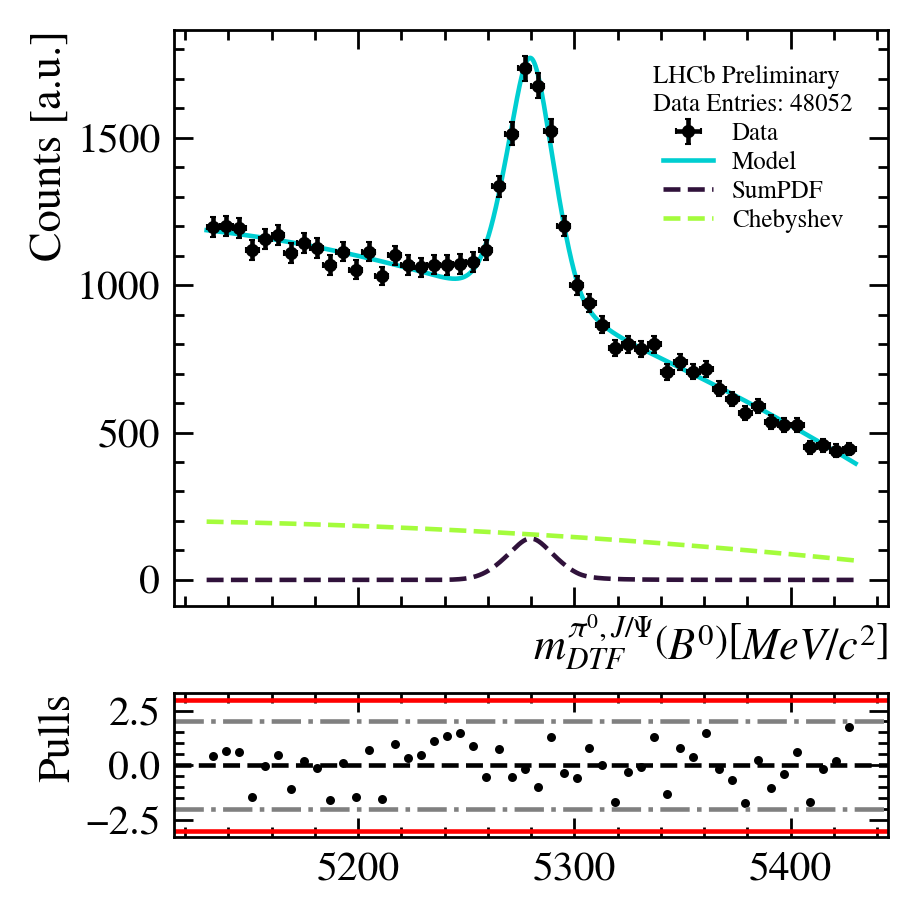
\includegraphics[width=\textwidth]{./OutputFiles/PNGPlots/PreliminaryFit/MVAScan/b1dfit_mva0.43_jpsichannel.png}
        \caption*{Preliminary fit for B (MVACut=0.43)}
        \label{fig:prefit_mvascan_mvacut040_b}
    \end{subfigure}
    \begin{subfigure}{0.49\textwidth}
        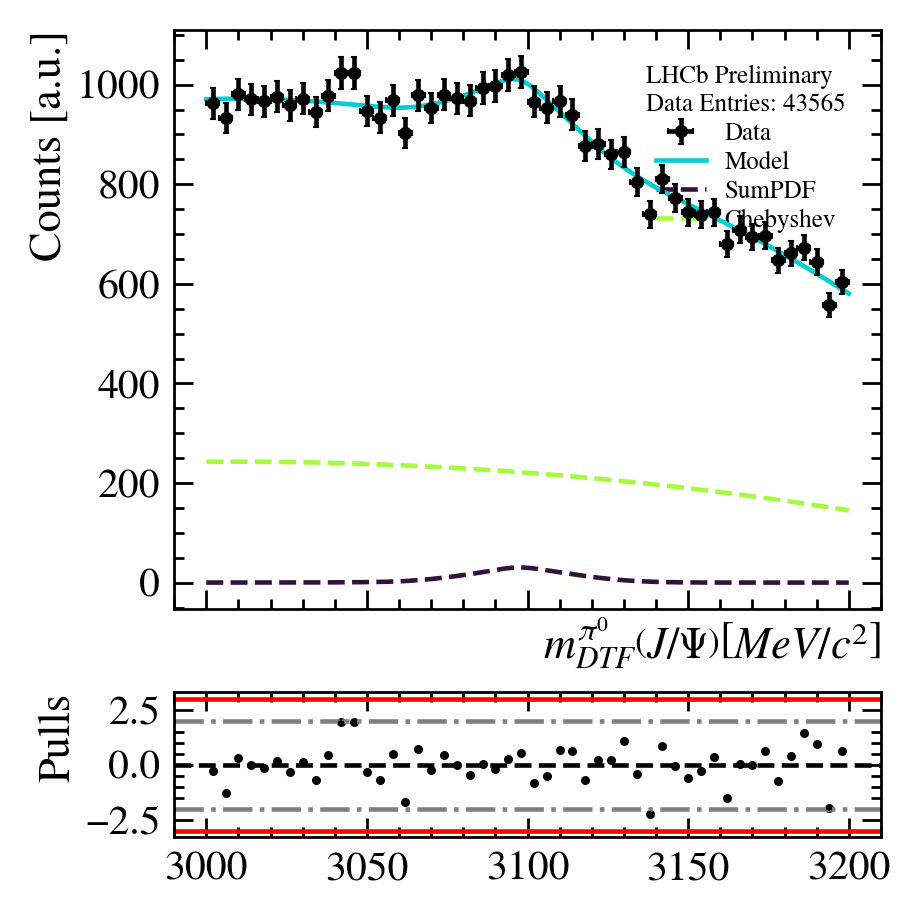
\includegraphics[width=\textwidth]{./OutputFiles/PNGPlots/PreliminaryFit/MVAScan/jpsi1dfit_mva0.43_jpsichannel.png}
        \caption*{Preliminary fit for $J/\psi$ (MVACut=0.43)}
        \label{fig:prefit_mvascan_mvacut040_b}
    \end{subfigure}
    \begin{subfigure}{0.49\textwidth}
        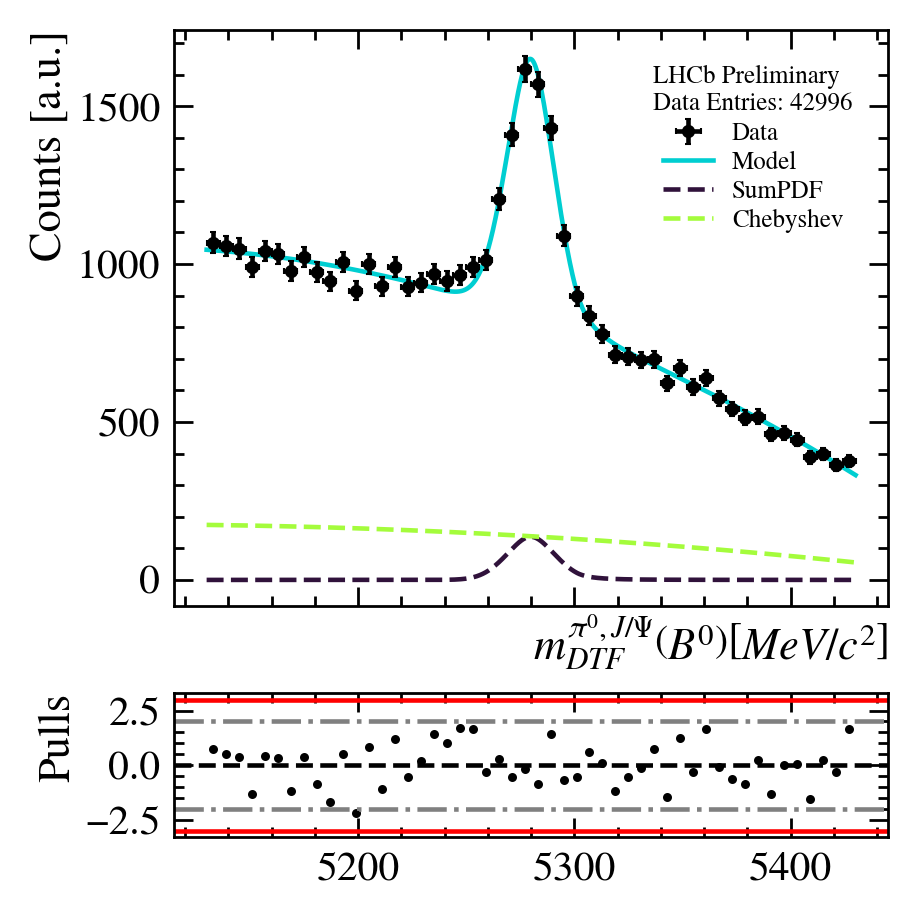
\includegraphics[width=\textwidth]{./OutputFiles/PNGPlots/PreliminaryFit/MVAScan/b1dfit_mva0.44_jpsichannel.png}
        \caption*{Preliminary fit for B (MVACut=0.44)}
        \label{fig:prefit_mvascan_mvacut040_b}
    \end{subfigure}
    \begin{subfigure}{0.49\textwidth}
        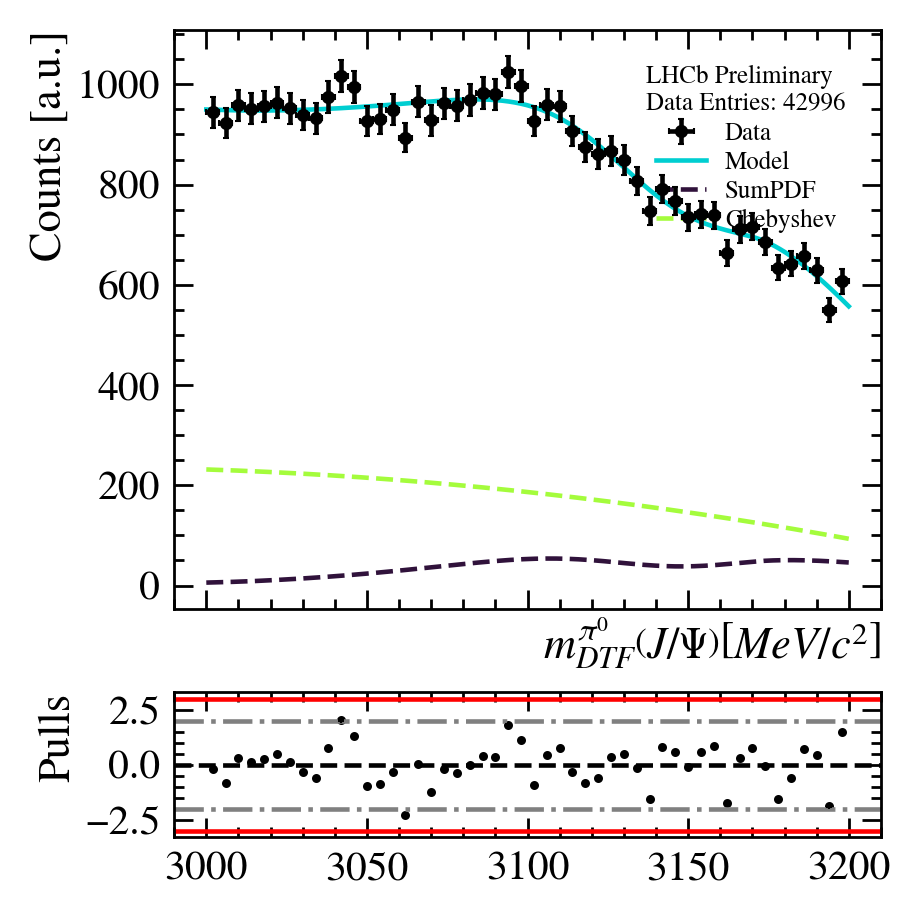
\includegraphics[width=\textwidth]{./OutputFiles/PNGPlots/PreliminaryFit/MVAScan/jpsi1dfit_mva0.44_jpsichannel.png}
        \caption*{Preliminary fit for $J/\psi$ (MVACut=0.44)}
        \label{fig:prefit_mvascan_mvacut040_b}
    \end{subfigure}
\end{figure}
\end{document}